\documentclass{article}
\usepackage[nonatbib]{project}
\usepackage{watml}

\usepackage[normalem]{ulem}
\usepackage{setspace}
% use Times
\usepackage{times}
% For figures
\usepackage{graphicx} % more modern
%\usepackage{epsfig} % less modern
%\usepackage{subfig} 

% path to figure folder
\graphicspath{{../fig/}}

% bib file for references
\addbibresmyce{project.bib}


\title{Predicting Plant Traits from Images Using ResNet50 and Ancillary Data}

\author{
	William Wang \\
	\texttt{w559wang@uwaterloo.ca} \\
	{\color{red} report due: August 12}
}

\begin{document}
\maketitle

\begin{abstract} 
This project addresses the challenge of predicting plant traits from citizen science photographs and ancillary data as part of the CS 480 Project Kaggle competition. I developed an iterative approach using ResNet50 for image feature extraction combined with ancillary data to predict six specific plant traits. My methodology evolved from an initial multi-output model to individual models for each trait, incorporating early stopping and hyperparameter tuning. The final approach achieved positive R scores for 5 out of 6 traits. Key challenges included dealing with non-converging models for certain traits and adapting to varied trait distributions. This report details my data preprocessing, model architecture, training process, and results analysis. My code is available within the submitted .zip file to Learn as a Jupyter Notebook along with the training logs detailing the training loss and validation loss across 30 epochs. The project highlights the potential and challenges of using deep learning for plant trait prediction from diverse data sources.
\end{abstract} 

\section{Introduction}
My project aimed to predict six plant traits (X4, X11, X18, X26, X50, and X3112) from citizen science photographs and ancillary data. Building on recent research by Schiller et al. (2021), I developed an iterative approach to model creation, prioritizing simplicity to mitigate overfitting.

My methodology centered on a pre-trained ResNet50 model for image feature extraction, integrated with ancillary environmental data. Initially, I attempted a single multi-output model, but later transitioned to individual models for each trait. This approach allowed me to leverage both visual and contextual information effectively.

Through this process, I achieved positive R scores for five out of the six traits (X4, X11, X26, X50, and X3112), with only X18 proving challenging to predict accurately. This report details my data preprocessing, model architecture, training process, and results analysis, highlighting both the potential and challenges of using deep learning for plant trait prediction.

\Cref{fig:trait_model_losses} summarizes the training and validation loss for all 6 models I trained to predict each plant trait.

\begin{figure*}[h]
\centering
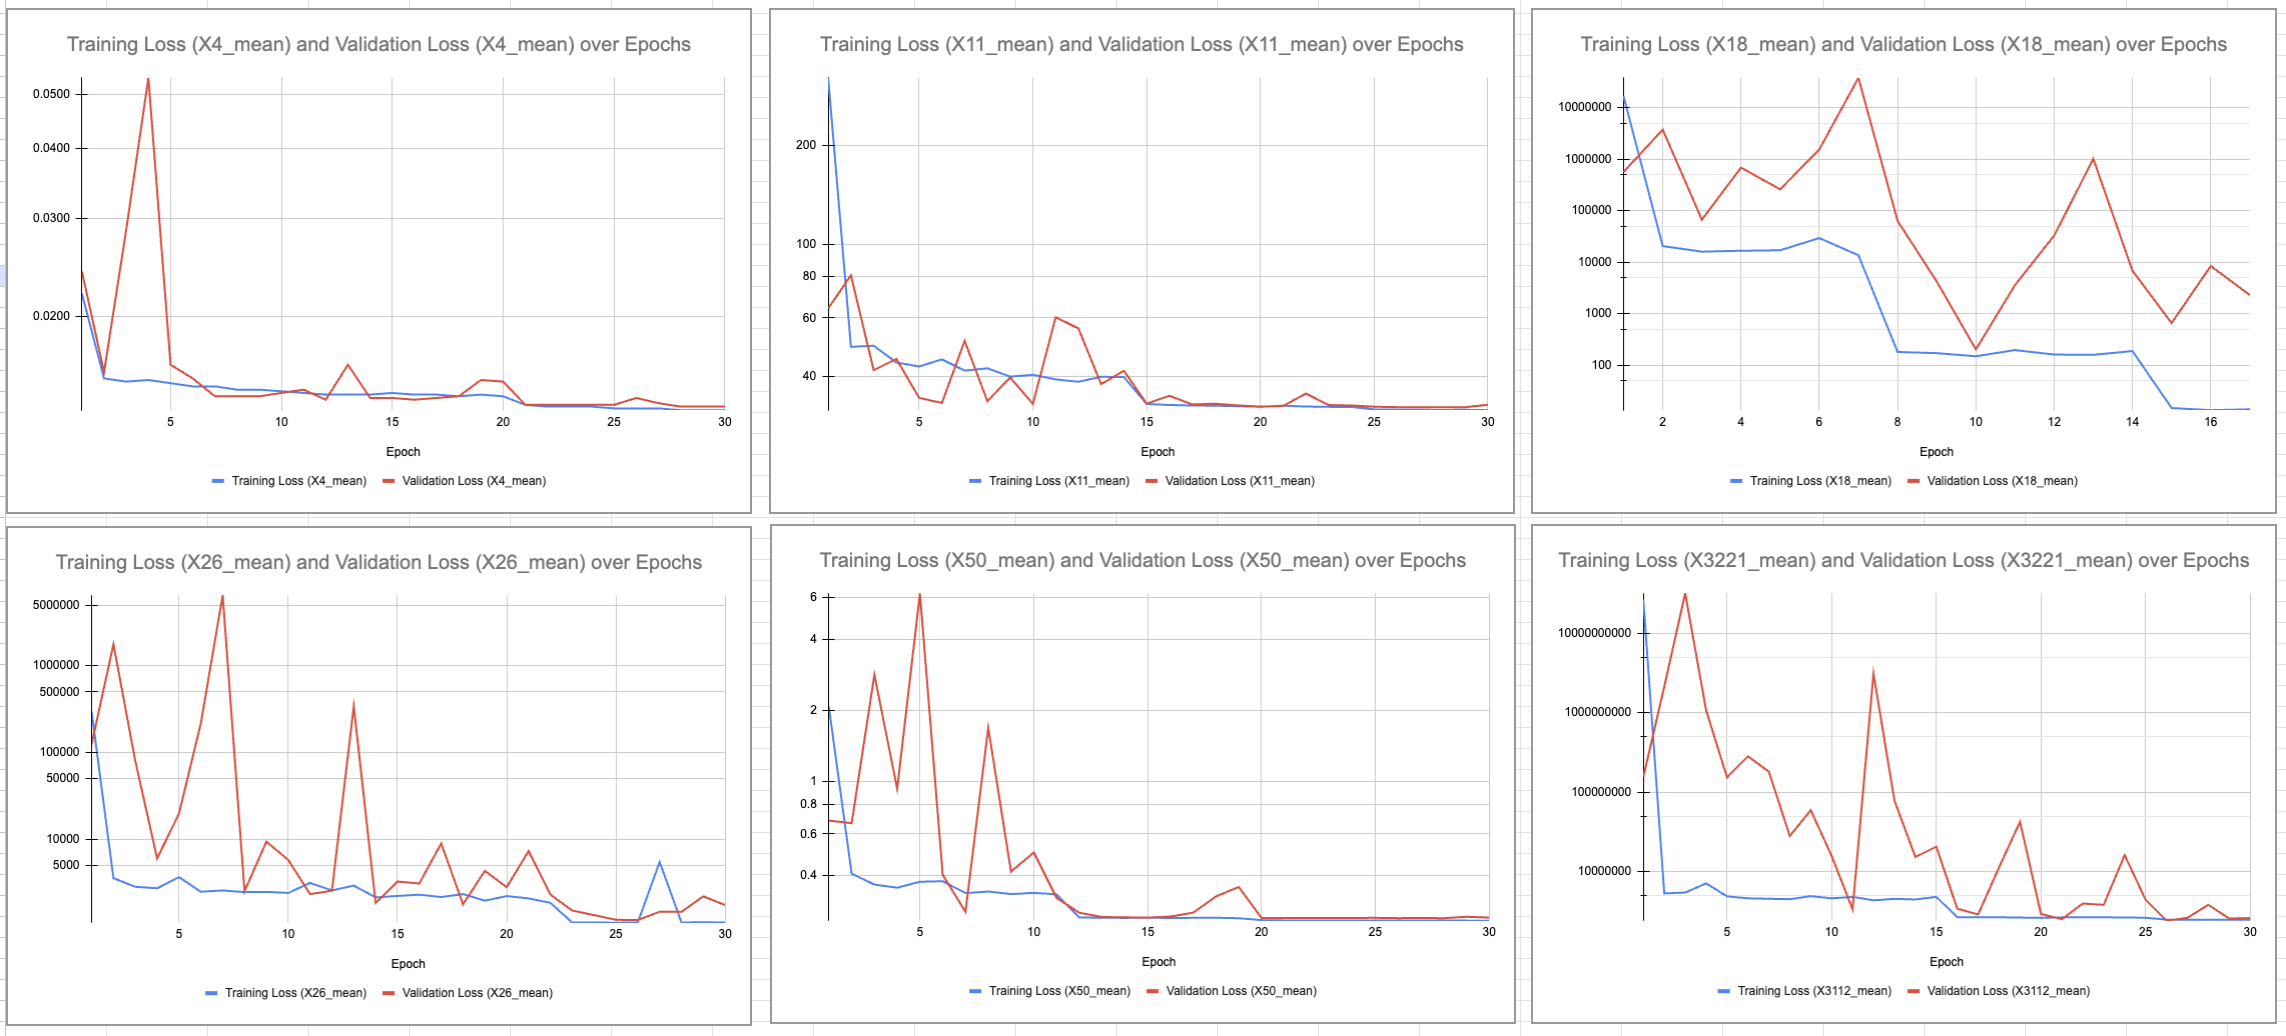
\includegraphics[width=1.0 \textwidth]{1_allLosses.png}
\caption{Training and validation loss curves over epochs for the six individual models predicting plant traits X4, X11, X18, X26, X50, and X3112. Each subplot represents a separate model's performance. Note that all models show convergence in their loss curves except for X18, which exhibits unstable behavior and fails to converge within the given number of epochs.}
\label{fig:trait_model_losses}
\end{figure*}

\section{Initial Approach}

My initial approach to this Kaggle project was guided by the principle of starting with the simplest possible model and increasing complexity only when necessary to mitigate overfitting. To begin, I conducted research by reviewing discussions on the course's Piazza forum, where I learned that pretrained ResNet models were yielding promising results for many students [1, 2]. 

Based on this information, I decided to use a pretrained ResNet model to extract features from the plant images. However, I hypothesized that the ancillary data provided in the dataset might also contain valuable information for predicting plant traits. To test this, I designed a model that combined the ResNet-extracted image features with the 163 additional data points from the ancillary data.

For the first version (v1) of my model, I created a single neural network that used the pretrained ResNet for image feature extraction, concatenated these features with the ancillary data, and then attempted to predict all six plant traits simultaneously through a shared set of fully connected layers. 

Unfortunately, this initial approach did not yield satisfactory results. The predictions generated by this model had a negative public score of -7.57886, performing much worse than a simple baseline model that predicted the mean value for each trait. This outcome suggested that the model was either underfitting due to insufficient complexity or overfitting to noise in the training data. 

\section{Improved Approach}

After the initial model's unsatisfactory performance, I revised my strategy to address the complexity of predicting multiple plant traits simultaneously. The key change was to train six separate models, each dedicated to predicting one of the six plant traits (X4, X11, X18, X26, X50, and X3112).

I began by training a model to predict trait X4. This single-trait model showed significant improvement, achieving a positive R score of 0.03063. Encouraged by this result, I applied the same architecture to create individual models for the remaining five traits.

Based on the convergence behavior observed in the X4 model, which stabilized around 20 epochs, I set the maximum number of epochs to 30 for all models. To prevent overfitting and optimize training time, I implemented early stopping with a patience of 7 epochs.

Figure \ref{fig:trait_model_losses} illustrates the training and validation loss curves for each of the six trait models.

The individual model approach proved successful for most traits, with models for X4, X11, X26, X50, and X3112 all showing convergence in their loss curves. However, the model for trait X18 exhibited unstable behavior and failed to converge before early stopping was activated at epoch 17.

To address the poor performance of the X18 model, I used the mean value of X18 from the training dataset as a baseline predictor for X18 predictions, achieving my best public score of 0.09733 on the Kaggle leaderboard.

\section{Technical Implementation}

\subsection{Preprocessing}

1. Image Preprocessing: Upscaled images to 224x224 pixels using bicubic interpolation, optimizing for ResNet performance [3]. Normalized pixel values using ImageNet-typical mean and standard deviation.
2. Ancillary Data Preprocessing: Removed outliers by filtering data outside 0.1th-98th percentiles for each trait. Applied StandardScaler for normalization, focusing model learning on representative data points and reducing skew from extreme values.
Copy

\subsection{Model Architecture}

The core of my approach is a neural network model that combines image features extracted by a pretrained ResNet50 with ancillary data to predict individual plant traits. The model architecture is designed to be simple yet effective, balancing the need for feature extraction with the goal of avoiding overfitting.  Key components of this architecture include:
\begin{enumerate}
    \item \textbf{ResNet50 Backbone}: 
    \begin{itemize}
        \item I use a pretrained ResNet50 model with the default weights as the backbone for image feature extraction.
        \item The final fully connected layer of ResNet50 is replaced with a new linear layer that outputs 256 features, allowing for more compact image representation.
    \end{itemize}
    
    \item \textbf{Feature Combination}:
    \begin{itemize}
        \item The 256 image features are concatenated with 163 ancillary data points, resulting in a 419-dimensional feature vector.
    \end{itemize}
    
    \item \textbf{Fully Connected Layers}:
    \begin{itemize}
        \item The combined features are passed through two fully connected layers:
        \begin{itemize}
            \item The first layer (fc1) reduces the dimensionality from 419 to 128, with a ReLU activation.
            \item The second layer (fc2) produces the final output, a single value representing the predicted trait.
        \end{itemize}
    \end{itemize}
    
    \item \textbf{Single Trait Prediction}:
    \begin{itemize}
        \item The model is designed to predict a single trait, aligning with my approach of training separate models for each trait.
    \end{itemize}
\end{enumerate}

This architecture offers several advantages:
\begin{itemize}
    \item It leverages transfer learning through the pretrained ResNet50, benefiting from features learned on a large dataset.
    \item The combination of image and ancillary data allows the model to utilize all available information.
    \item The simplicity of the fully connected layers helps prevent overfitting while still allowing the model to learn non-linear relationships in the data.
\end{itemize}

\section{Analysis and Experimentation}

To further analyze results, I graphed the distribution of training traits versus predicted traits. As seen in Figures \ref{fig:train_dist} and \ref{fig:pred_dist} in the Appendix, the distributions of values my model predicted were Gaussian for all traits. However, only three traits (X4, X11, X50) appeared to be Gaussian in distribution in the training dataset, with the other three (X18, X26, X3112) appearing exponential.

It appears my model performed well on the traits with Gaussian distributions (X4, X11, X50) but struggled with predicting traits whose distributions were exponential (X18, X26, X3112).

\subsection{Model Complexity Experiment}

I hypothesized that my model of two fully connected layers might not be complex enough to capture the intricacy of the input data. To test this, I experimented with training models with three and four layers using a smaller training dataset for trait X11. The results were as follows:

\begin{table}[h]
    \centering
    \begin{tabular}{|c|c|c|}
        \hline
        Model & Training Loss (Epoch 15) & Validation Loss \\
        \hline
        2 Layers (Original) & 39.4057 & 37.0834 \\
        3 Layers & 46.0228 & 48.3218 \\
        4 Layers & 640.3750 & 1223.9818 \\
        \hline
    \end{tabular}
    \caption{Comparison of Model Performance with Different Layer Counts at Epoch 15}
    \label{tab:model_comparison}
\end{table}

As shown in Table \ref{tab:model_comparison}, the training and validation losses in each case were much higher compared to my original models trained with two fully connected layers, indicating that increasing model complexity did not improve performance for this particular task with a limited training and validation dataset.

\section{Conclusion}

This project has been an illuminating journey into the complexities of training AI models, particularly in the domain of plant trait prediction. Several key insights have emerged from this experience:

\subsection{Complexity and Experimentation}

The process of developing an effective AI model is both intimidating and exhilarating. The sheer number of parameters that can be tweaked and the myriad directions one can explore in model architecture and training strategies present an almost infinite space for experimentation. This project, being my first foray into training an AI model without the scaffolding of assignment instructions, has been both overwhelming but also an invaluable learning experience.

\subsection{Computational Demands}

One of the most significant realizations was the substantial computational resources required for training complex models. Even after separating the models for each trait, each training session consumed approximately an hour on my personal computer, or six hours in total for all six traits. This necessitated leaving the system running overnight to experiment with fresh sets of parameters, highlighting the importance of efficient time planning in machine learning projects.

\subsection{Future Directions}

For future improvement, I identified several avenues for future exploration:

\begin{itemize}
    \item \textbf{Model Architecture}: Further experimentation with different layer configurations and model depths could potentially yield improved performance. Time constraints limited the extent of this exploration in the current project as I only had time to experiment with a reduced dataset.
    
    \item \textbf{Data Preprocessing}: Normalizing ancillary and label values using StandardScaler; Investigating more sophisticated data transformation techniques, particularly for traits with non-Gaussian distributions, could enhance model accuracy.
    
    \item \textbf{Feature Engineering}: Deeper analysis of the relationships between ancillary data and plant traits might reveal more informative input features.
    
    \item \textbf{Ensemble Methods}: Exploring the combination of multiple models or techniques could potentially leverage the strengths of different approaches.
\end{itemize}

\subsection{Achievements}

In conclusion, despite the challenges encountered, the project achieved a significant milestone by attaining positive R-scores for five out of the six plant traits. This experiment underscores the potential of machine learning in botanical research and provides a good starting point for future refinements.





\newpage

\section{Appendix}
\begin{figure}[h]
    \centering
    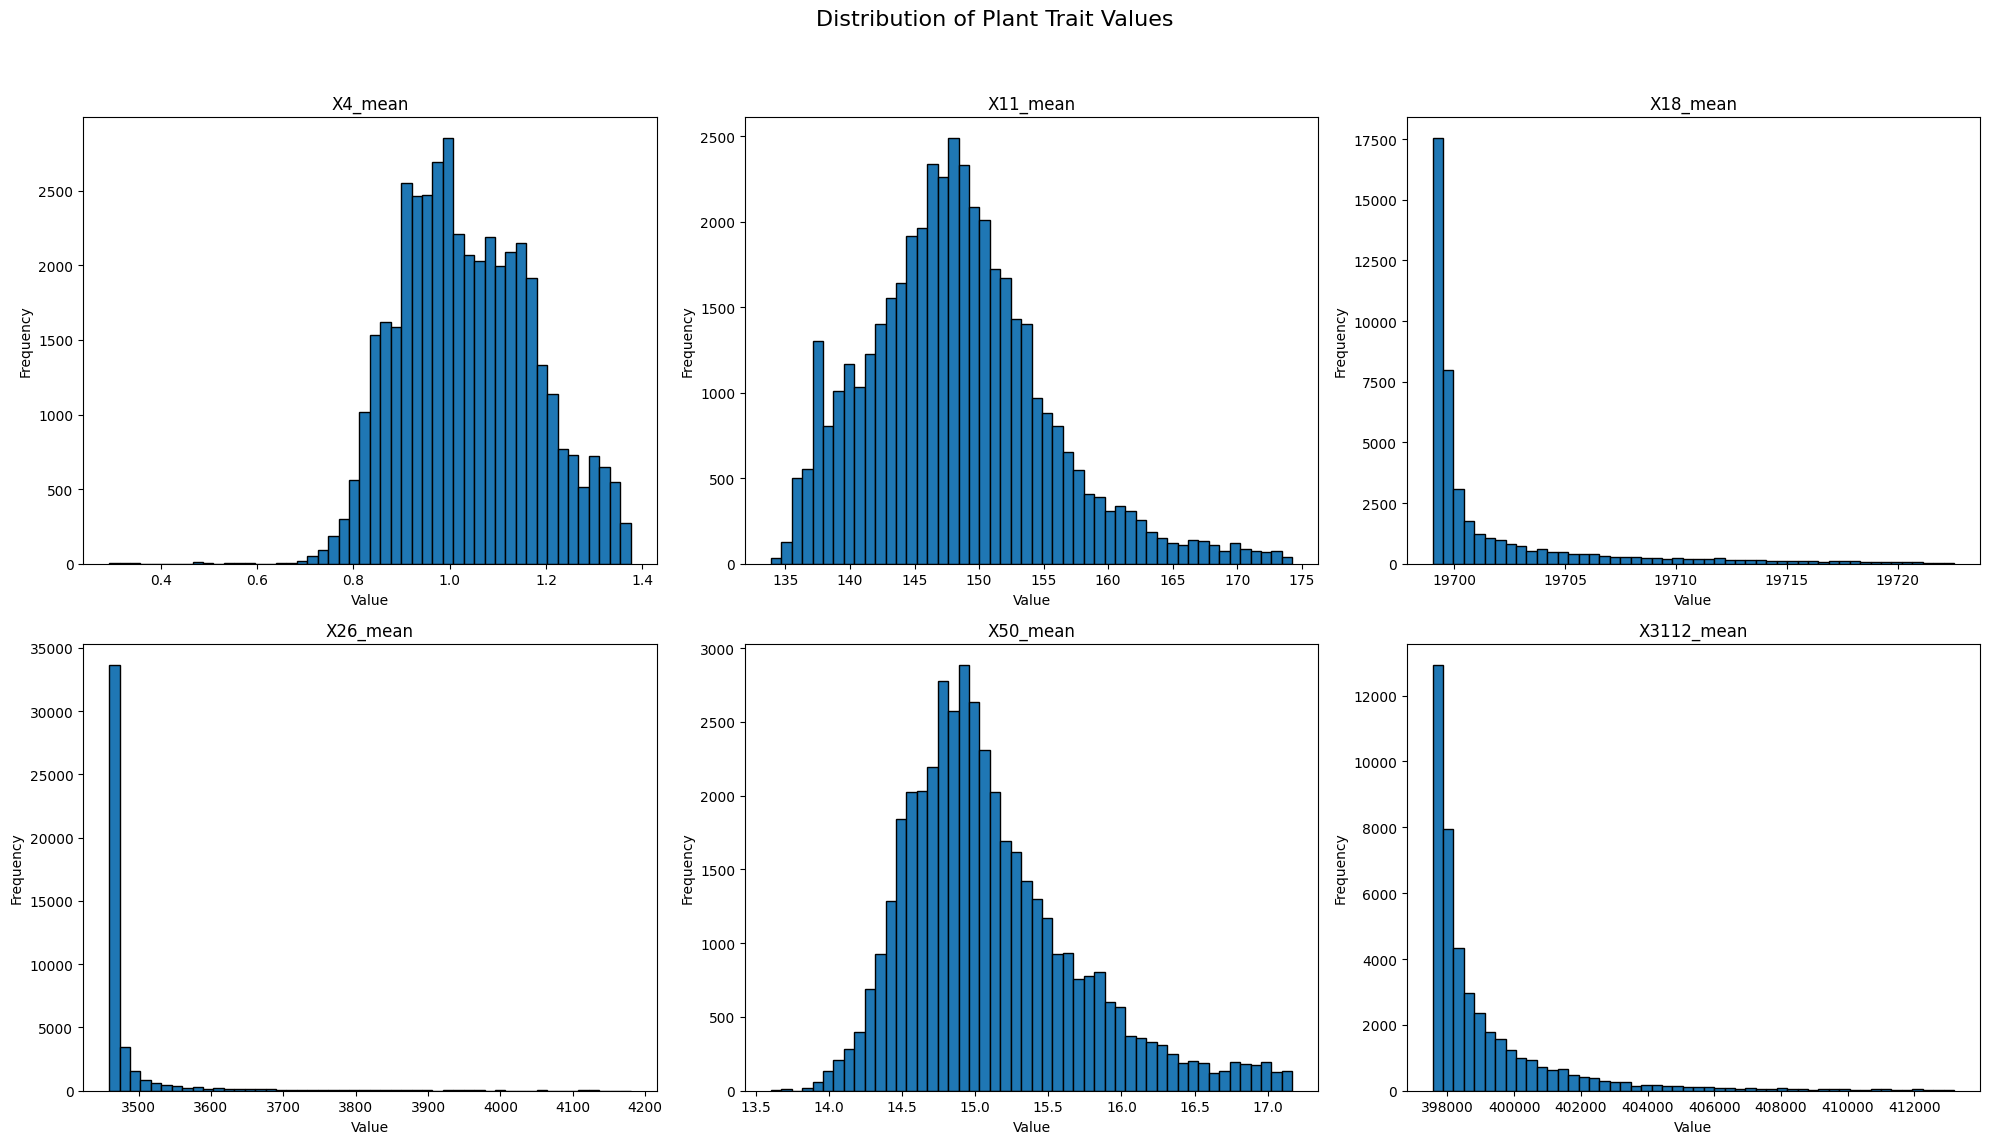
\includegraphics[width=\textwidth]{train_distribution.png}
    \caption{Distribution of Plant Trait Values in Training Data}
    \label{fig:train_dist}
\end{figure}

\begin{figure}[h]
    \centering
    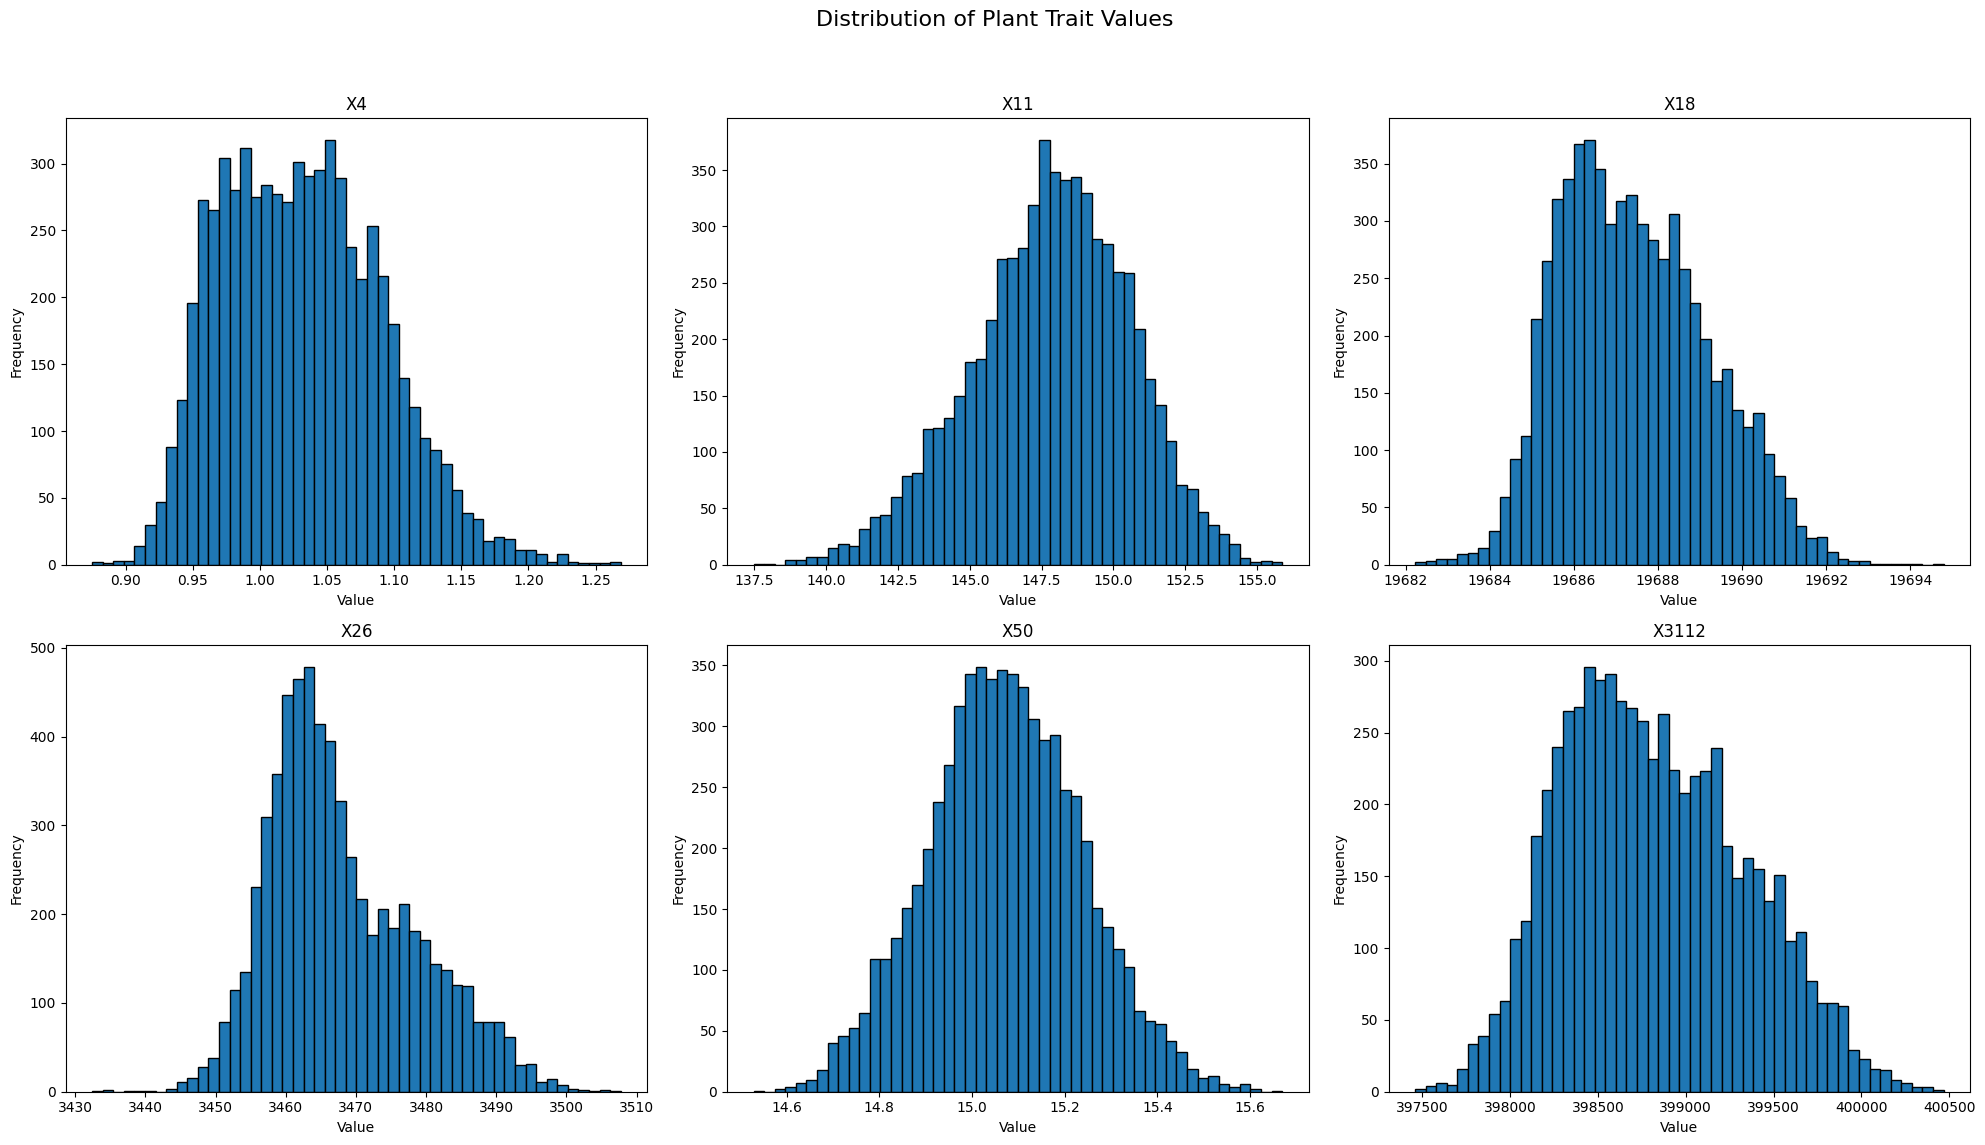
\includegraphics[width=\textwidth]{predicted_distribution.png}
    \caption{Distribution of Predicted Plant Trait Values}
    \label{fig:pred_dist}
\end{figure}

\section*{Acknowledgement}

I extend my gratitude to the students on Piazza for their collaborative spirit and to the instructors for their guidance and support throughout this course!

This challenging course has been an incredibly rewarding experience, and I'm grateful for the opportunity to have completed it successfully.

\nocite{*}
\printbibliography[title=References]


\end{document}